\upaper{41}{ФИЗИЧЕСКИЕ АСПЕКТЫ ЛОКАЛЬНОЙ ВСЕЛЕННОЙ}
\uminitoc{ЦЕНТРЫ МОЩИ НЕБАДОНА}
\uminitoc{ФИЗИЧЕСКИЕ РЕГУЛЯТОРЫ САТАНИИ}
\uminitoc{НАШИ ЗВЁЗДНЫЕ СОСЕДИ}
\uminitoc{ПЛОТНОСТЬ СОЛНЦА}
\uminitoc{СОЛНЕЧНОЕ ИЗЛУЧЕНИЕ}
\uminitoc{КАЛЬЦИЙ --- КОСМИЧЕСКИЙ СТРАННИК}
\uminitoc{ИСТОЧНИКИ СОЛНЕЧНОЙ ЭНЕРГИИ}
\uminitoc{СОЛНЕЧНО-ЭНЕРГЕТИЧЕСКИЕ РЕАКЦИИ}
\uminitoc{СТАБИЛЬНОСТЬ СОЛНЦА}
\uminitoc{ПРОИСХОЖДЕНИЕ ОБИТАЕМЫХ МИРОВ}
\author{Архангел}
\vs p041 0:1 Характерным пространственным феноменом, отделяющим каждое локальное творение от всех остальных, является присутствие Созидательного Духа. Весь Небадон совершенно пронизан пространственным присутствием Божественной Служительницы Спасограда, и это присутствие так же определённо исчезает у внешних границ нашей локальной вселенной. То, что пронизано Материнским Духом нашей локальной вселенной, \bibemph{есть} Небадон; то, что выходит за пределы его пространственного присутствия, находится за пределами Небадона, являясь вненебадонскими пространственными областями сверхвселенной Орвонтон~--- другими локальными вселенными.
\vs p041 0:2 \pc Хотя административная организация большой вселенной раскрывает чёткое разделение между правительствами центральной, сверх- и локальной вселенных, и хотя эти деления астрономически соответствуют пространственному разграничению Хавоны и семи сверхвселенных, между локальными творениями таких чётких линий физической демаркации не существует. Даже большие и малые сектора Орвонтона (для нас) чётко различимы, но определить физические границы локальных вселенных не так-то просто. Это связано с тем, что эти локальные творения административно организованы в соответствии с определёнными \bibemph{созидательными} принципами, определяющими сегментацию общего энергетического заряда сверхвселенной, тогда как их физические компоненты, сферы пространства~--- солнца, тёмные острова, планеты и т.\,д.~--- происходят преимущественно из туманностей, а те астрономически появляются в соответствии с определёнными \bibemph{предсозидательными} (трансцендентными) планами Зодчих Главной Вселенной.
\vs p041 0:3 Одна или несколько, и даже много, таких туманностей могут быть заключены в пределах одной локальной вселенной. Так, Небадон был физически образован из звёздного и планетарного потомства Андроновера и других туманностей. Сферы Небадона происходят от различных туманностей, однако все они обладали определённой минимальной общностью пространственного движения, которое было скорректировано разумными усилиями управляющих мощью таким образом, чтобы создать наше нынешнее скопление пространственных тел, движущихся как одно целое по орбитам сверхвселенной.
\vs p041 0:4 Таково строение локального звёздного облака Небадон, которое сегодня обращается по всё более устойчивой орбите вокруг находящегося в Стрельце центра того малого сектора Орвонтона, к которому принадлежит наше локальное творение.
\usection{ЦЕНТРЫ МОЩИ НЕБАДОНА}
\vs p041 1:1 Начало спиральным и другим туманностям~--- материнским дискам сфер пространства~--- кладут Райские организаторы силы; и вслед за эволюцией небулярной гравитационной реакции их функции передаются центрам мощи и физическим регуляторам, которые с этого момента берут на себя полную ответственность за управление физической эволюцией последующих поколений звёздного и планетарного потомства. Этот физический надзор за предвселенной Небадон после прибытия нашего Сына Создателя был сразу же скоординирован с его планом организации вселенной. Во владениях этого Райского Сына Бога Верховные Центры Мощи и Главные Физические Регуляторы сотрудничали с появившимися позже Управляющими Моронтийной Мощью и другими, с целью создания того обширного комплекса линий связи, энергетических контуров и магистралей мощи, которые прочно связывают разнообразные пространственные тела Небадона в единую интегрированную административную единицу.
\vs p041 1:2 Сто Верховных Центров Мощи четвёртой категории постоянно закреплены за нашей локальной вселенной. Эти существа принимают входящие линии энергии из центров третьей категории Уверсы и передают пониженные и модифицированные контуры центрам мощи наших созвездий и систем. В совокупности эти центры мощи образуют живую систему контроля и выравнивания, которая работает для поддержания баланса и распределения энергий, которые иначе были бы флуктуирующими и переменными. Однако центры мощи не связаны с кратковременными и локальными энергетическими потрясениями, такими как солнечные пятна и системные электрические возмущения; свет и электричество не являются основными энергиями пространства; они являются вторичными и побочными проявлениями.
\vs p041 1:3 Сто центров локальной вселенной размещены на Спасограде, где они функционируют в самом энергетическом центре этой сферы. Архитектурные сферы, такие как Спасоград, Эденция и Иерусем, освещаются, обогреваются и снабжаются энергией методами, которые делают их совершенно независимыми от солнц пространства. Эти сферы были сконструированы~--- созданы по плану~--- центрами мощи и физическими регуляторами таким образом, чтобы оказывать мощное влияние на распределение энергии. Сосредоточивая свою деятельность на таких фокусных точках энергетического контроля, центры мощи своим живым присутствием направляют и перераспределяют физические энергии пространства. И эти энергетические контуры лежат в основе всех физико\hyp{}материальных и моронтийно\hyp{}духовных явлений.
\vs p041 1:4 Каждому из первичных подразделений Небадона~--- ста созвездий~--- назначено по десять Верховных Центров Мощи пятой категории. В вашем созвездии Норлатиадек они расположены не на столичной сфере, а в центре огромной звёздной системы, образующей физическое ядро созвездия. На Эденции расположено десять соответствующих механических регуляторов и десять франдаланков, которые находятся в идеальной и постоянной связи с ближайшими центрами мощи.
\vs p041 1:5 Точно в фокусе гравитации каждой локальной системы находится по одному Верховному Центру Мощи шестой категории. В системе Сатания назначенный центр мощи занимает тёмный остров пространства, расположенный в астрономическом центре системы. Многие из этих тёмных островов представляют собой огромные генераторы [dynamos], мобилизующие и направляющие определённые энергии пространства, и эти естественные обстоятельства эффективно используются Центром Мощи Сатании, чья живая масса функционирует в качестве связи с высшими центрами, направляя потоки более материализованной мощи Главным Физическим Регуляторам на эволюционных планетах пространства.
\usection{ФИЗИЧЕСКИЕ РЕГУЛЯТОРЫ САТАНИИ}
\vs p041 2:1 Хотя Главные Физические Регуляторы служат вместе с центрами мощи по всей большой вселенной, их функции в локальной системе, такой как Сатания, более просты для понимания. Сатания является одной из 100 локальных систем, составляющих административную организацию созвездия Норлатиадек, а её непосредственными соседями являются системы Сандматия, Ассунция, Порогия, Сортория, Рантулия и Глантония. Системы Норлатиадека во многих отношениях отличаются друг от друга, но все они являются эволюционными и развивающимися, в чём весьма схожи с Сатанией.
\vs p041 2:2 Сама Сатания состоит из более чем 7\,000 астрономических групп или физических систем, лишь немногие из которых имеют происхождение, подобное вашей Солнечной системе. Астрономический центр Сатании представляет собой огромный тёмный остров пространства, расположенный вместе с сопровождающими его сферами недалеко от центра правительства системы.
\vs p041 2:3 \pc Если не считать присутствия назначенного центра мощи, управление всей физико\hyp{}энергетической системой Сатании сосредоточено на Иерусеме. Главный Физический Регулятор, размещённый на этой столичной сфере, работает согласованно с центром мощи системы, выступая в качестве начальника связи инспекторов мощи, имеющих свой центр на Иерусеме и действующих по всей локальной системе.
\vs p041 2:4 Заключением в контуры и перераспределением [channelizing] энергии руководят 500\,000 живых и разумных манипуляторов энергии, разбросанных по всей Сатании. Благодаря действию таких физических регуляторов, управляющие центры мощи осуществляют полный и совершенный контроль над большинством основных энергий пространства, в том числе излучений сильно нагретых сфер и тёмных энерго\hyp{}заряженных сфер. Эта группа живых существ может мобилизовывать, преобразовывать, превращать, манипулировать и передавать почти все виды физической энергии организованного пространства.
\vs p041 2:5 Жизни присуща способность к мобилизации и трансмутации всеобщей энергии. Тебе знаком механизм растительной жизни, посредством которого материальная энергия света преобразуется в разнообразные проявления растительного царства. Ты также знаешь кое-что о методе, посредством которого эта растительная энергия может быть преобразована в явления животной деятельности, но ты практически ничего не знаешь о методе управляющих мощью и физических регуляторов, наделённых способностью мобилазиции, преобразования, направления и концентрации разнообразных видов энергии пространства.
\vs p041 2:6 \pc Эти существа энергетического царства не имеют прямого отношения к энергии как составляющему фактору живых созданий, даже к области физиологической химии. Иногда они занимаются физическими предпосылками жизни, разработкой тех энергетических систем, которые могут служить физическими проводниками жизненных энергий элементарных материальных организмов. В некотором смысле физические регуляторы связаны с предшествующими жизни проявлениями материальной энергии, так же как адъютанты разумо\hyp{}духи связаны с преддуховными функциями материального разума.
\vs p041 2:7 \pc Эти разумные создания, связанные с контролем мощи и управлением энергии, должны приспосабливать свои методы на каждой сфере в соответствии с физическим строением и архитектурой данной планеты. Они неизменно используют расчёты и выводы своего штата физиков и других технических консультантов относительно локального влияния сильно нагретых солнц и других типов сверхзаряженных звёзд. Необходимо также считаться с огромными холодными и тёмными гигантами пространства и роящимися облаками звёздной пыли; вся эта материя связана с практическими проблемами манипулирования энергией.
\vs p041 2:8 Управление мощью\hyp{}энергией эволюционных обитаемых миров является обязанностью Главных Физических Регуляторов, но эти существа не несут ответственности за все энергетические сбои на Урантии. Существует целый ряд причин для таких нарушений, некоторые из которых находятся вне области и контроля физических хранителей. Урантия находится на линиях колоссальных энергий,~--- маленькая планета в контуре чудовищных масс, и локальные регуляторы иногда привлекают огромное число существ своей категории в усилии уравновесить эти линии энергии. Они довольно хорошо справляются с физическими контурами Сатании, однако сталкиваются с трудностями, изолируя от мощных токов Норлатиадека.
\usection{НАШИ ЗВЁЗДНЫЕ СОСЕДИ}
\vs p041 3:1 Более 2\,000 сверкающих солнц\fnst{Сфера радиусом 65 световых лет с центром в Урантии содержит около 2\,000 звёзд. Если предположить однородную плотность звёзд по всей Сатании, то можно сделать вывод, что размер Сатании не может значительно превышать 130 световых лет.} изливают свет и энергию в Сатании, и ваше собственное солнце представляет собой обычный пылающий шар. Из тридцати ближайших солнц только три ярче вашего\fnst{Тридцать ближайших звёзд находятся в сфере радиусом 12,6 световых лет, а три звезды, которые ярче нашей следующие: $\alpha$~Центавра (4,35 св. лет), Сириус (8,57 св. лет) и Процион (11,4 св. лет). Это те самые три звезды, которые упомянты в книге Дж.~Джинса \cite{Jeans1}, являющейся одним из человеческих источников данного документа Откровения.}. Вселенские Управляющие Мощью инициируют специальные потоки энергии, протекающие между отдельными звёздами и соответствующими системами. Эти солнечные печи вместе с тёмными гигантами пространства служат центрам мощи и физическим регуляторам в качестве промежуточных станций для эффективной концентрации и направления энергетических контуров материальных творений.
\vs p041 3:2 Солнца Небадона мало чем отличаются от солнц других вселенных. Материальный состав всех солнц, тёмных островов, планет и спутников, даже метеоров, совершенно одинаков. Диаметр таких солнц составляет в среднем около $1,6\times 10^6$\,км, а у вашего солнечного шара он немного меньше\fnst{Современное значение диаметра Солнца $1,392684\times 10^6$\,км.}. Диаметр крупнейшей звезды во вселенной~--- звёздного облака Антарес~--- около $10^9$\,км, что в 680 раз превосходит диаметр вашего солнца. В него можно было бы вместить около 207 миллионов ваших солнц, и ещё осталось бы место\fnst{Американский текст 1955 года в данном параграфе содержит сразу две ошибки: во-первых, приводится неверное значение диаметра звезды Антарес (450 диаметров Солнца) и, во-вторых, утверждается, что объём Антареса превосходит солнечный в 60 миллионов раз. Эти два утверждения несовместимы при условии применимости геометрии Евклида в окрестности звезды Антарес и в окрестности Солнца. Возможность согласования этих утверждений с помощью неевклидовой геометрии в рамках общей теории относительности Эйнштейна была исследована в 2012 году (см.\,\cite{Aivazian1}) и была отвергнута, ибо она приводит к выводу о громадной плотности звезды Антарес, недопустимой для звёзд данного типа. Эта загадка оставалась нерешённой до 2018 года, когда я обнаружил точное место в книге Дж.~Джинса \cite{Jeans1}, неверное понимание которого автором данного параграфа Откровения явилось причиной противоречия. На странице 183 \cite{Jeans1} читаем: Indeed the largest yet known (Antares) has a diameter 450 times that of the sun or about 400 million miles. We could pack about 60 million suns inside it, and there would still be room to spare. А теперь сравним это с американским текстом Откровения, почти дословно дублирующем первое предложение Джинса, но существенно отличающемся от второго: The largest star in the universe, the stellar cloud Antares, is four hundred and fifty times the diameter of your sun and is sixty million times its volume. В книге Джинса идёт речь об \bibemph{упаковке} множества идентичных сфер внутри сферы б\'ольшего диаметра, что вовсе не то же самое, что отношение \bibemph{объёмов} этих сфер. Утверждение в книге Джинса безупречно как с астрономической (согласно имевшимся на тот момент данным), так и с математической, точек зрения. Но автор данного текста Откровения (вероятно, доктор Уильям Садлер) перепутал упаковку сфер с отношением их объёмов, тем самым введя противоречие в американский вариант текста Откровения. В тексте Британского издания обе эти ошибки были исправлены. При этом было использовано то же самое значение упаковочного коэффициента, на которое опирался Джинс в своей книге, то есть 65.7\%, а не оптимальное значение 74\%, которое было получено Гауссом уже в XIX веке. Для диаметра звезды Антарес было использовано современное значение из \cite{Ohnaka1}. Я доложил об этой находке и исправлении соответствующих ошибок в Откровении 24 марта 2018 года, запись доклада доступна здесь: \myurl{https://youtu.be/LSbfi2BWqN8}.}. Однако существует более чем достаточно пространства для размещения всех этих огромных солнц. У них относительно столько же места в пространстве, сколько было бы у дюжины апельсинов\fnst{В оригинале у Эддингтона ``тридцать мячей для крикета'' вместо ``дюжины апельсинов''.}, если бы они двигались внутри Урантии и если бы планета представляла собой полый шар.\tunemarkup{pictures}{\begin{figure}[H]\centering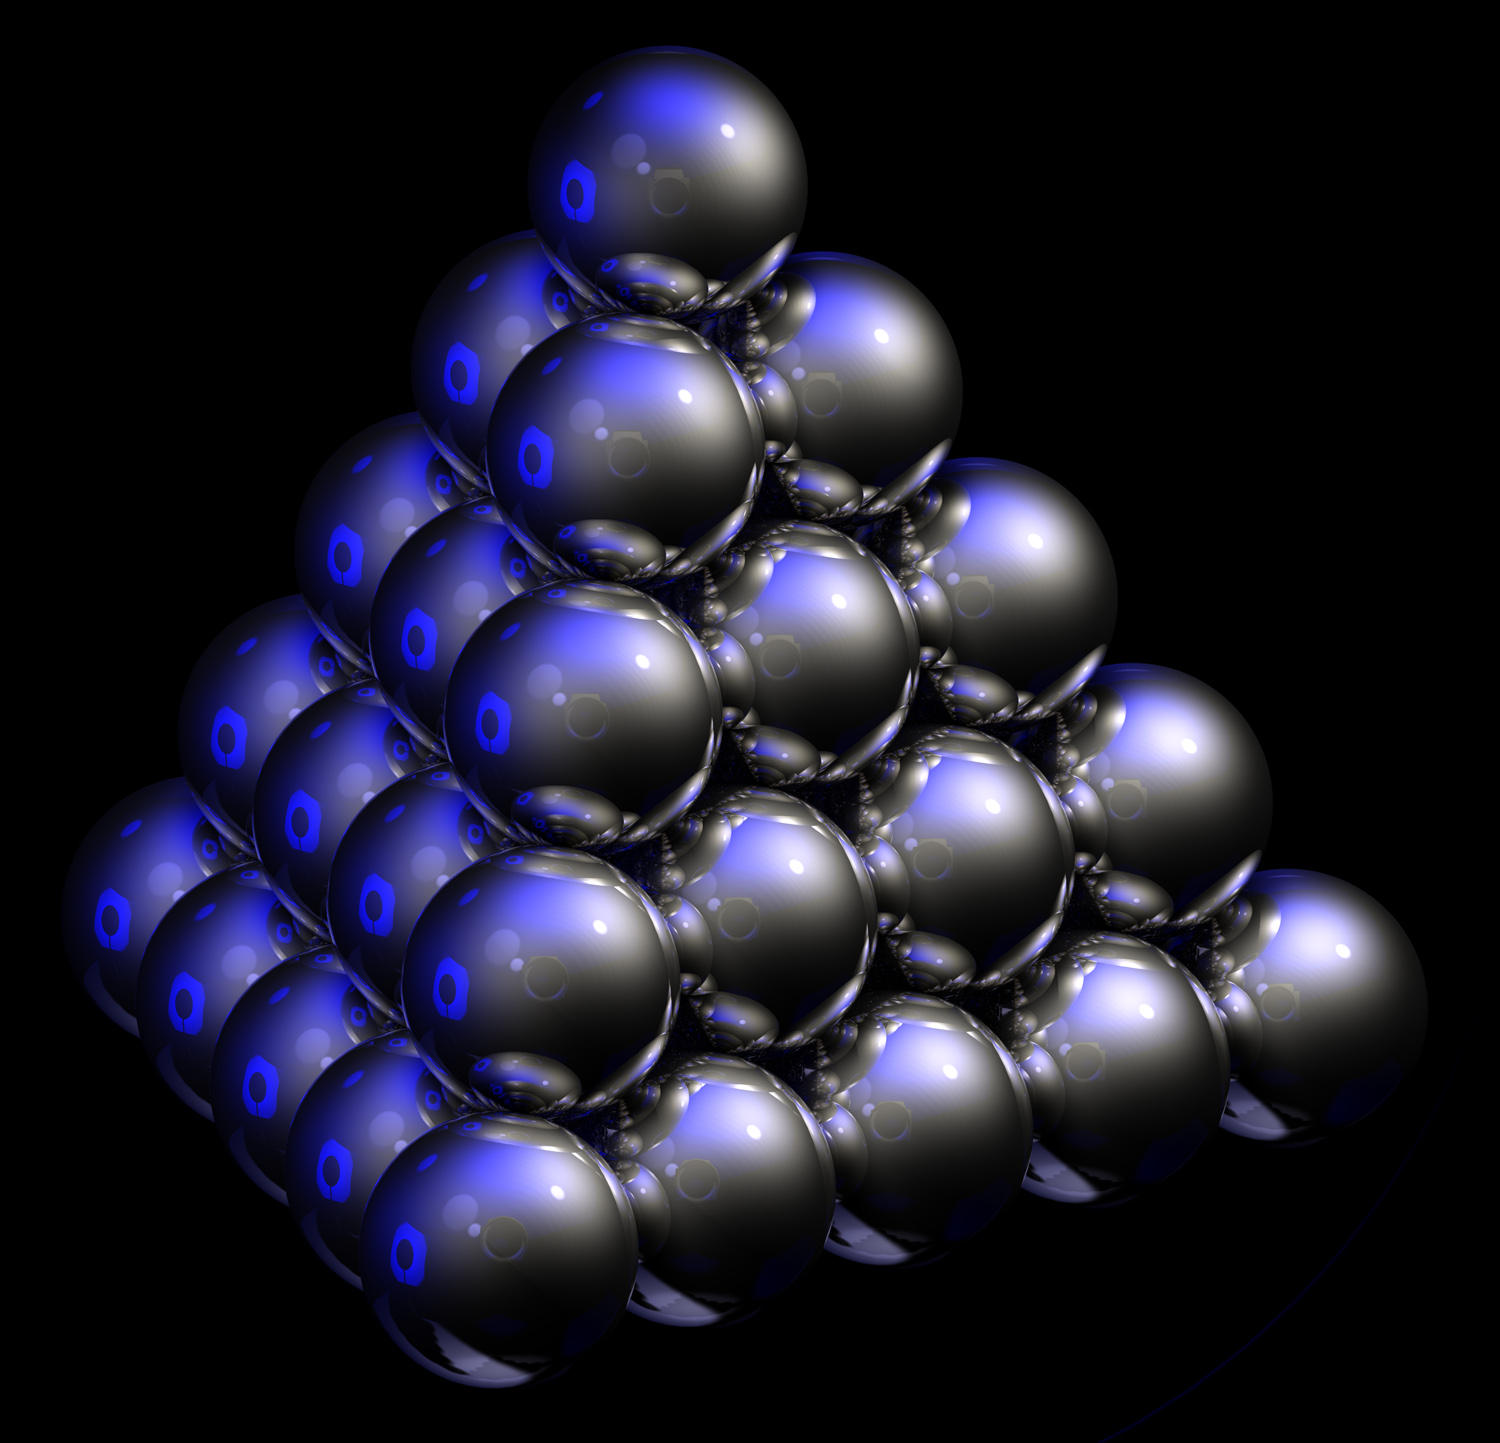
\includegraphics[width=0.95\columnwidth]{images/sphere-packing.jpg}\caption{Плотная упаковка сфер.}\end{figure}}
\vs p041 3:3 \pc Когда слишком большие солнца выбрасываются из материнского диска туманности, то вскоре они распадаются или образуют двойные звёзды. Все солнца изначально пребывают в истинно газообразном состоянии, хотя впоследствии они могут временно существовать в полужидком состоянии. Когда ваше солнце достигло этого квазижидкого состояния, соответствующего давлению сверхгаза\fnst{Понятие <<сверхгаза>>, введённое Эддингтоном, определяется ниже (см.\,\bibref[41:4.3]{p041 4:3}) как почти полностью ионизованная плазма.}, оно не было достаточно большим, чтобы разделиться по экватору, что является одним из типов формирования двойных звёзд.
\vs p041 3:4 В случае размеров, в десять раз меньших, чем размер вашего солнца, эти огненные сферы быстро сжимаются, уплотняются и остывают. Когда же их размеры превышают его в 30 раз~--- а точнее, в 30 раз превышают общее количество фактического материала,~--- солнца легко расщепляются на два отдельных тела, либо становясь центрами новых систем, либо оставаясь в пределах взаимного гравитационного влияния и вращаясь вокруг общего центра, как это присуще одному из типов двойных звёзд.
\vs p041 3:5 \pc 
\vs p041 3:6 \pc 
\vs p041 3:7 
\vs p041 3:8 \pc 
\vs p041 3:9 
\vs p041 3:10 
\usection{ПЛОТНОСТЬ СОЛНЦА}
\vs p041 4:1 
\vs p041 4:2 \pc 
\vs p041 4:3 \pc 
\vs p041 4:4 
\vs p041 4:5 
\vs p041 4:6 
\vs p041 4:7 
\usection{СОЛНЕЧНОЕ ИЗЛУЧЕНИЕ}
\vs p041 5:1 
\vs p041 5:2 
\vs p041 5:3 
\vs p041 5:4 
\vs p041 5:5 
\vs p041 5:6 \pc 
\vs p041 5:7 \pc 
\vs p041 5:8 
\usection{КАЛЬЦИЙ --- КОСМИЧЕСКИЙ СТРАННИК}
\vs p041 6:1 
\vs p041 6:2 
\vs p041 6:3 \pc 
\vs p041 6:4 
\vs p041 6:5 
\vs p041 6:6 \pc 
\vs p041 6:7 \pc 
\usection{ИСТОЧНИКИ СОЛНЕЧНОЙ ЭНЕРГИИ}
\vs p041 7:1 
\vs p041 7:2 
\vs p041 7:3 \pc 
\vs p041 7:4 
\vs p041 7:5 
\vs p041 7:6 
\vs p041 7:7 
\vs p041 7:8 
\vs p041 7:9 
\vs p041 7:10 
\vs p041 7:11 \pc 
\vs p041 7:12 \pc 
\vs p041 7:13 
\vs p041 7:14 \pc 
\vs p041 7:15 
\usection{СОЛНЕЧНО-ЭНЕРГЕТИЧЕСКИЕ РЕАКЦИИ}
\vs p041 8:1 
\vs p041 8:2 \pc 
\vs p041 8:3 \pc 
\vs p041 8:4 
\usection{СТАБИЛЬНОСТЬ СОЛНЦА}
\vs p041 9:1 
\vs p041 9:2 \pc 
\vs p041 9:3 \pc 
\vs p041 9:4 
\vs p041 9:5 
\usection{ПРОИСХОЖДЕНИЕ ОБИТАЕМЫХ МИРОВ}
\vs p041 10:1 
\vs p041 10:2 
\vs p041 10:3 \pc 
\vs p041 10:4 
\vs p041 10:5 \pc 
\vsetoff
\vs p041 10:6 
\quizlink
\begin{thebibliography}{100}
\bibitem{Eddington1}
A.S.~Eddington.
{``Stars and Atoms''}
{\em Oxford: Clarendon Press}, 1927.
\bibitem{Jeans1}
J.~Jeans.
{``Through Space and Time''}
{\em Cambridge: University Press}, 1934.
\bibitem{Aivazian1}
T.~Aivazian.
{``The Volume of Antares''}
{\em \myurl{http://www.bibles.org.uk/articles/T.Aivazian-The-Volume-of-Antares.pdf}}, 2012.
\bibitem{Ohnaka1}
Keiichi Ohnaka, Karl-Heinz Hofmann, Dieter Schertl, Gerd Weigelt, Carlo Baffa, Alain Chelli, Romain Petrov, Sylvie Robbe-Dubois.
{``High spectral resolution imaging of the dynamical atmosphere of the red supergiant Antares in the CO first overtone lines with VLTI/AMBER''}
{\em \myurl{https://arxiv.org/abs/1304.4800}}, 2013.
\end{thebibliography}
